% Answer key for sedimentation.tex. The figure and the numerical checks of every result
% here are made by scripts/sedimentation.py. Equation numbers are Gardiner, 2nd ed.
\documentclass[11pt]{article}

\usepackage[letterpaper,margin=1in]{geometry}
\usepackage[T1]{fontenc}
\usepackage{lmodern}
\usepackage{microtype}
\usepackage{amsmath,amssymb,mathtools}
\usepackage[dvipsnames]{xcolor}
\usepackage{graphicx}
\usepackage{enumitem}
\usepackage[most]{tcolorbox}
\usepackage[colorlinks=true,urlcolor=PineGreen,linkcolor=PineGreen]{hyperref}

\graphicspath{{figures/}}
\setlength{\parindent}{0pt}
\setlength{\parskip}{6pt}
\setlist{itemsep=3pt,topsep=2pt}

\newcommand{\dd}{\mathrm{d}}
\newcommand{\avg}[1]{\langle #1\rangle}

\newcommand{\sheethead}[1]{%
  {\sffamily\Large\color{PineGreen}Sedimentation in a box}\par\vspace{2pt}
  {\sffamily\small Answer key\hfill #1}\par\vspace{-7pt}
  \rule{\textwidth}{0.5pt}\par\vspace{2pt}}
\newcommand{\exsec}[1]{\par\vspace{6pt}{\sffamily\bfseries\large\color{PineGreen}#1}\par\vspace{-2pt}}

\newtcolorbox{keyresults}{enhanced, colback=black!3, colframe=black!35, boxrule=0.4pt, arc=1pt,
  left=6pt, right=6pt, top=4pt, bottom=4pt, colbacktitle=black!10, coltitle=black,
  fonttitle=\bfseries\small, title={Key results}}

\begin{document}

\sheethead{Journal club}

$\dd x=-v\,\dd t+\sqrt D\,\dd W$ on $0<x<L$, with $h=D/2v=k_BT/mg$, $k_n=n\pi/L$, and $B=D$ the variance per unit
time. Closed cell: reflecting walls. Sticky cell: absorbing walls. Equation numbers are Gardiner, 2nd edition.

\begin{keyresults}
\small
\vspace{-6pt}
\begin{alignat*}{2}
  &\text{forward equation:} &\quad& \partial_tp=v\,\partial_xp+\tfrac12D\,\partial_x^2p=-\partial_xJ,\qquad
     J=-vp-\tfrac12D\,\partial_xp \\
  &\text{closed, stationary:} &\quad& p_s=\frac{e^{-x/h}}{h\,(1-e^{-L/h})},\qquad \avg x_s=h-\frac L{e^{L/h}-1} \\
  &\text{both cells:} &\quad& \lambda_n=\frac{v^2}{2D}+\frac{n^2\pi^2D}{2L^2}\ (n\ge1);\quad
     \text{the closed cell also has }\lambda_0=0 \\
  &\text{closed modes:} &\quad& Q_n=e^{x/2h}\varphi_n,\quad P_n=\frac{e^{-x/2h}\varphi_n}{N_n},\quad\text{with}\quad
     \varphi_n=\cos k_nx-\frac{\sin k_nx}{2hk_n} \\
  &\text{normalisation:} &\quad& N_n=\int_0^L\varphi_n^2\,\dd x=\frac L2\Bigl(1+\frac1{4h^2k_n^2}\Bigr) \\
  &\text{sticky modes:} &\quad& Q_n=e^{x/2h}\sin k_nx,\quad P_n=\frac2L\,e^{-x/2h}\sin k_nx,\quad
     q=\frac{(2h)^{-2}+k_1^2}{k_1\,(1+e^{-L/2h})}\,e^{-x/2h}\sin k_1x \\
  &\text{sticking:} &\quad& \pi_L=\frac{e^{x_0/h}-1}{e^{L/h}-1},\qquad T=\frac{x_0-L\,\pi_L(x_0)}v \\
  &\text{from the QSD:} &\quad& \avg T=\frac1{\lambda_1},\qquad \Pr(\text{ceiling})=\frac1{1+e^{L/2h}} \\
  &\text{the map:} &\quad& J\bigl[P_n^{\rm closed}\bigr]=\tfrac12Dk_n\,P_n^{\rm sticky},\qquad
     P_n^{\rm closed}=\partial_xJ\bigl[P_n^{\rm closed}\bigr]/\lambda_n
\end{alignat*}
\end{keyresults}

% =========================================================
\exsec{(a) The closed cell: find the stationary state}
\textbf{1.} $A=-v$, $B=D$, so $\partial_tp=v\,\partial_xp+\frac12D\,\partial_x^2p=-\partial_xJ$ with
$J=-vp-\frac12D\,\partial_xp$. Hard walls reflect: $J(0,t)=J(L,t)=0$.

\textbf{2.} $2A/B=-2v/D=-1/h$, so (5.2.39) gives $p_s\propto e^{-x/h}$, and
\[ \boxed{\;p_s(x)=\frac{e^{-x/h}}{h\,(1-e^{-L/h})},\qquad h=\frac D{2v}=\frac{2k_BT/\gamma}{2mg/\gamma}=\frac{k_BT}{mg}\;} \]
This is the Boltzmann factor $e^{-mgx/k_BT}$. Friction sets how fast the particle moves, not where it ends up in
equilibrium, so $\gamma$ cancels between $v$ and $D$.

\textbf{3.} $m=\frac43\pi r^3\Delta\rho=5.2\times10^{-16}$\,kg, $mg=5.1\times10^{-15}$\,N, so $h\approx0.8\,\mu$m:
the colloid's atmosphere is a micron thick, and the cell is tall on that scale. With $\gamma=6\pi\eta r$ and
$\eta=1.0$\,mPa\,s, the settling speed is $v\approx0.55\,\mu$m/s, so $h/v\approx1.4$\,s.

\textbf{4.} $\avg x_s=\int_0^Lx\,p_s\,\dd x=h-\dfrac L{e^{L/h}-1}$.
For $L\ll h$, expanding gives $\avg x_s\simeq\frac L2-\frac{L^2}{12h}$: nearly uniform. For $L\gg h$,
$\avg x_s\to h$: the floor's atmosphere, which does not feel the ceiling.

% =========================================================
\exsec{(b) The closed cell: find the modes}
\textbf{1.} $e^{ax}$ needs $\frac12Da^2-va+\lambda=0$, so $a=[v\pm\sqrt{v^2-2D\lambda}\,]/D=1/2h\pm ik$ with
$\lambda=v^2/2D+\frac12Dk^2$. Take $Q=e^{x/2h}(\cos kx+c\sin kx)$. $Q'(0)=0$ gives $c=-1/2hk$, and then
\[ Q'(L)=-e^{L/2h}\Bigl(k+\frac1{4h^2k}\Bigr)\sin kL=0\quad\Longrightarrow\quad k_n=\frac{n\pi}L. \]
For real $a$, put $k=i\kappa$: the condition becomes $(\kappa-1/4h^2\kappa)\sinh\kappa L=0$, so $\kappa=1/2h$. That is
$\lambda=0$ with $Q=e^{x/2h}(\cosh\frac x{2h}-\sinh\frac x{2h})=1$, the stationary mode. There are no others.

\textbf{2.} With $\int p_sQ_nQ_m\,\dd x=\delta_{nm}N_n/[h(1-e^{-L/h})]$, the normalised pair is
\[ Q_n=e^{x/2h}\varphi_n,\qquad P_n=\frac{e^{-x/2h}\varphi_n}{N_n},\qquad
   \varphi_n=\cos k_nx-\frac{\sin k_nx}{2hk_n},\qquad N_n=\frac L2\Bigl(1+\frac1{4h^2k_n^2}\Bigr). \]
Since $J[p_s]=0$, $J[p_sQ]=-\frac12D\,p_s\,Q'$, which vanishes wherever $Q'=0$. The backward condition (5.2.69) is
the forward one in disguise.

\textbf{3.} $\lambda_1=v^2/2D+\pi^2D/2L^2$. The second term is free diffusion across the cell, the gap of the talk's
box. The first is added to every mode by the drift, whatever $L$: it is $v/4h$, the rate of settling through a few
gravitational lengths. For $L\gg h$ it dominates, and $1/\lambda_1\simeq4h/v$, independent of $L$.

\textbf{4.} At $L=20h$: $\lambda_1=(0.25+0.025)\,v/h$, so $1/\lambda_1\approx3.6\,h/v$, while settling from the
ceiling takes about $20\,h/v$. The expansion explains it:
\[ p(x,t\,|\,x_0,0)-p_s(x)=e^{(x_0-x)/2h}\sum_{n\ge1}\frac{\varphi_n(x)\,\varphi_n(x_0)}{N_n}\,e^{-\lambda_nt}. \]
For $x_0=L$ and $x$ near the floor, the prefactor is $e^{L/2h}=e^{10}\approx2\times10^4$, while $p_s\sim1/h$. The
modes cancel almost exactly at first, which is how the density near the floor starts at zero. The deviation is
small only once $e^{L/2h}e^{-\lambda_1t}\ll1$, that is, after $t\approx(L/2h)/\lambda_1\approx2L/v$: of the order
of the settling time. The gap sets the final exponential approach, not when it begins. Large coefficients like these
are the price of a non-symmetric operator. In the symmetrised variables $e^{\pm x/2h}$ is removed, and nothing is
paradoxical.

% =========================================================
\exsec{(c) Make the walls sticky}
\textbf{1.} A stationary state has constant $J$, so $-vp-\frac12Dp'=J$, with solution
$p=Ce^{-x/h}-(J/v)(1-e^{-x/h})$. $p(0)=0$ gives $C=0$, and $p(L)=0$ then gives $J=0$, so $p=0$. Every particle
eventually sticks.

\textbf{2.} $Q=e^{x/2h}(\alpha\cos kx+\beta\sin kx)$ with $Q(0)=0$ gives $\alpha=0$. $Q(L)=0$ gives $\sin kL=0$, so
$k_n=n\pi/L$ again. Real $a$ fails, because $\sinh\kappa L\ne0$. So
\[ \boxed{\;Q_n=e^{x/2h}\sin k_nx,\qquad \lambda_n=\frac{v^2}{2D}+\frac{n^2\pi^2D}{2L^2},\qquad n\ge1\;} \]
exactly the nonzero rates of the closed cell. Only $\lambda_0=0$ is lost (panel c). Part (e) explains why.

\textbf{3.} $p_sQ_n\propto e^{-x/2h}\sin k_nx$. Trying $e^{ax}$ in the forward equation $vP'+\frac12DP''=-\lambda P$
gives $a=-1/2h\pm ik$ with the same $\lambda$, and $p=0$ at the walls holds. Gardiner's (5.2.91) keeps the
reflecting $p_s$ for absorbing walls. Since $\int p_sQ_nQ_m\,\dd x\propto\int_0^L\sin k_nx\sin k_mx\,\dd x$, the
normalised pair is $Q_n=e^{x/2h}\sin k_nx$ and $P_n=\frac2L\,e^{-x/2h}\sin k_nx$.

\textbf{4.} $q=P_1/\int P_1\,\dd x$. With the integral in the hint,
\[ \boxed{\;q(x)=\frac{(2h)^{-2}+k_1^2}{k_1\,(1+e^{-L/2h})}\;e^{-x/2h}\sin\frac{\pi x}L\;} \]
Its peak is where $\tan(\pi x^*/L)=2\pi h/L$: $x^*\approx1.7h$ for $L=8h$, and $x^*\to2h$ for $L\gg h$
(panel a). Why higher than $p_s$: $q\propto p_sQ_1$, and $Q_1(x_0)$ is the long-time survival weight,
$S(t\,|\,x_0)\simeq Q_1(x_0)\int P_1\,\dd x\;e^{-\lambda_1t}$. Particles low down soon touch the floor, so the
survivors come from higher up, and the weight $e^{x/2h}$ turns $e^{-x/h}$ into $e^{-x/2h}$.

\textbf{5.} The approach rate is $\lambda_2-\lambda_1=3\pi^2D/2L^2$. The drift adds the same $v^2/2D$ to every mode,
so it cancels in every difference. Gravity speeds up sticking, but the survivors' shape settles by diffusion across
the whole cell. For $L\gg h$, $\lambda_2-\lambda_1\ll\lambda_1$: most particles stick before the survivors' shape
settles, the opposite of metastability. Panel (b) is at $L=8h$, where the two rates are comparable.

\begin{figure}[h]
  \centering
  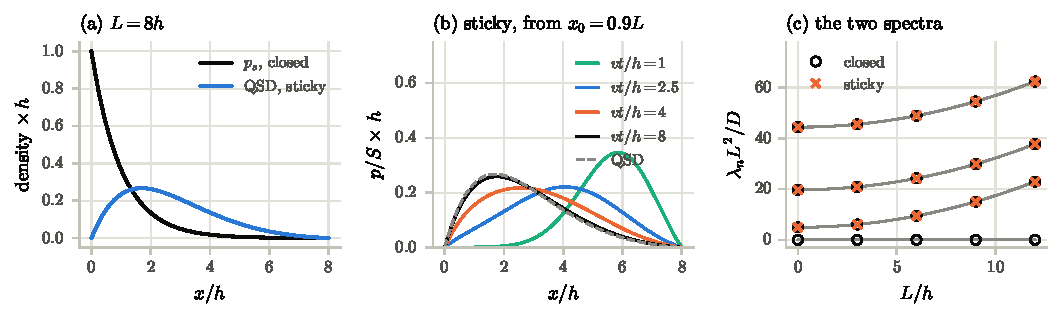
\includegraphics[width=\textwidth]{sed_modes.pdf}
  \caption{\small (a) Barometric $p_s$ of the closed cell and the QSD of the sticky cell, $L=8h$. (b) Sticky cell,
  $L=8h$, particles released at $x_0=0.9L$: the density conditioned on survival, from the mode sum, settles onto the
  QSD. (c) Rates against $L/h$: curves are $\lambda_n$ for $n=0,\dots,3$; markers are eigenvalues of
  finite-difference matrices for the closed cell (circles) and the sticky cell (crosses).}
\end{figure}

% =========================================================
\exsec{(d) Where and when does it stick?}
\textbf{1.} With $\psi=e^{-x/h}$, the corrected (5.2.189)--(5.2.190) give
$\pi_L=\int_0^{x_0}e^{y/h}\dd y\big/\!\int_0^Le^{y/h}\dd y=(e^{x_0/h}-1)/(e^{L/h}-1)$. It solves
$-v\pi'+\frac12D\pi''=0$, $\pi(0)=0$, $\pi(L)=1$, as (5.2.186)--(5.2.187) require. For $L\gg h$,
$\pi_L\simeq e^{-(L-x_0)/h}$: only particles that start within a few $h$ of the ceiling have a fair chance. It is
the barometric factor again.

\textbf{2.} The general solution of $-vT'+\frac12DT''=-1$ is $T=x/v+c_1+c_2e^{x/h}$, and $T(0)=T(L)=0$ give
\[ \boxed{\;T(x_0)=\frac{x_0-L\,\pi_L(x_0)}v\;} \]
For $L\gg h$, away from the ceiling, $\pi_L\approx0$ and $T\approx x_0/v$: the time to fall to the floor.

\textbf{3.} Started as the QSD, $p(x,t)=q(x)\,e^{-\lambda_1t}$ exactly, so $S(t)=e^{-\lambda_1t}$: the time to
stick is exponential with mean $1/\lambda_1$. At the walls $q=0$, so $J=-\frac12Dq'$. Writing $q=C\,e^{-x/2h}\sin
k_1x$,
\[ J(0)=-\tfrac12DCk_1\ \ (\text{down, out through the floor}),\qquad J(L)=+\tfrac12DCk_1\,e^{-L/2h}. \]
The total outflux is $\frac12DCk_1(1+e^{-L/2h})=\frac12D\bigl[(2h)^{-2}+k_1^2\bigr]=\lambda_1$. The ceiling's share
is $e^{-L/2h}/(1+e^{-L/2h})=1/(1+e^{L/2h})$ at every moment, and so overall: $1.8\%$ for $L=8h$.

\textbf{4.} Averaging over starting points drawn from $q$:
\[ \int_0^Lq\,T\,\dd x=\frac1{\lambda_1},\qquad \int_0^Lq\,\pi_L\,\dd x=\frac1{1+e^{L/2h}}. \]
Both are hard integrals made easy (the script checks them).

% =========================================================
\exsec{(e) Optional: why the spectrum survived}
\textbf{1.} With constant $A$ and $D$,
$\partial_tJ=A\,\partial_tp-\frac12D\,\partial_x\partial_tp=-A\,\partial_xJ+\frac12D\,\partial_x^2J$: the same forward
equation.

\textbf{2.} In the closed cell $J=0$ at both walls at all times, so $J$ is a solution of the sticky-cell problem. A
mode $P_ne^{-\lambda_nt}$ has current $J[P_n]e^{-\lambda_nt}$, a sticky mode with the same $\lambda_n$, unless the
current vanishes. Explicitly, with $\varphi_n'=-k_n\sin k_nx-\frac1{2h}\cos k_nx$,
\[ J[P_n^{\rm closed}]=-\frac D{2N_n}\,e^{-x/2h}\Bigl(\frac{\varphi_n}{2h}+\varphi_n'\Bigr)
   =\frac D{2N_n}\Bigl(k_n+\frac1{4h^2k_n}\Bigr)e^{-x/2h}\sin k_nx=\tfrac12Dk_n\,P_n^{\rm sticky}. \]
The stationary mode has $J[p_s]\equiv0$: its current is not a mode, and so $\lambda_0$ has no partner.

\textbf{3.} Let $\mathcal L\tilde p=-A\tilde p\,'+\frac12D\tilde p\,''=-\lambda\tilde p$ with $\tilde p=0$ at the
walls, and set $P=\tilde p\,'/\lambda$. Then $J[P]=(A\tilde p\,'-\frac12D\tilde p\,'')/\lambda=-\mathcal L\tilde
p/\lambda=\tilde p$, which vanishes at the walls, and $\mathcal LP=-\partial_xJ[P]=-\tilde p\,'=-\lambda P$. So
$P$ is a closed-cell mode. The two maps are inverse to each other, and the spectra agree except for $\lambda_0$.
In particular $P_n^{\rm closed}=\partial_xJ[P_n^{\rm closed}]/\lambda_n$.

\textbf{4.} Constant $A$ was used to move $A$ through $\partial_x$. With $A=-U'(x)$ and constant $D$,
$\partial_tJ=-A\,\partial_xJ+\frac12D\,\partial_x^2J$. That is the \emph{backward} equation of the reflected
potential $-U$, with $J=0$ at the walls. So the closed problem in $U$ and the sticky problem in $-U$ share every
nonzero rate. These are the supersymmetric partners of quantum mechanics, here in imaginary time. For constant
drift, reflecting the potential changes nothing, since $\lambda_n$ depends only on $v^2$.

% =========================================================
\exsec{For the discussion}
\begin{itemize}
  \item \textbf{Survivors feel no gravity.} Weighting paths by their chance of surviving forever (Doob's
        $h$-transform, with $h=Q_1$) adds the drift $D\,\partial_x\ln Q_1=v+(\pi D/L)\cot(\pi x/L)$. The particle
        conditioned never to stick has drift $(\pi D/L)\cot(\pi x/L)$, whatever $v$, and stationary density
        $P_1Q_1\propto\sin^2(\pi x/L)$, symmetric. The QSD is lopsided because it describes particles that have
        survived \emph{so far}, not forever.
  \item \textbf{Same spectrum, different physics.} In the closed cell, $\lambda_1$ is the rate of approach to
        equilibrium. In the sticky cell, the same number is the rate of loss.
  \item \textbf{Checks.} \texttt{scripts/sedimentation.py} checks $p_s$, $\avg x_s$ and the silica numbers; the
        residuals, boundary conditions and biorthogonality of both sets of modes; both spectra against
        finite-difference matrices; the QSD, its peak and its currents; survival against a finite-difference
        solution; $\pi_L$, $T$ and the two averages in (d); the map in (e); and the conditioned drift above, at
        $L/h=2$, $10$ and $0.33$.
\end{itemize}

\end{document}
